%\documentclass[compress,dvips,xcolor=table]{beamer}
\usepackage{etex}
%\documentclass{article}
%\usepackage{beamerarticle}
%\usepackage{pstricks,pst-node} % PSTricks package
%\usepackage[turkish]{babel}
\usepackage{tikz}
\usetikzlibrary{positioning,shapes,fit,arrows,graphs,shadows}
\usepackage[utf8]{inputenc}
\usepackage{listings}
\usepackage{multicol}
%\includeonlyframes{current}

\def\circtxt#1{$\mathalpha \bigcirc \mkern-13mu \mathtt #1$}

\mode<article>
{
  \usepackage{fullpage}
  \usepackage{pgf}
  \usepackage{hyperref}
}

\mode<presentation>
{
  \usetheme{metuceng}

%  \setbeamercovered{transparent}
}


\title{Programming Language Concepts}
\subtitle{Type Systems}
\author{Onur Tolga Şehitoğlu}
\institute[METU]{Computer Engineering}
\subject{Type Systems}
\date{}
	\titlegraphic{\insertmetutitle\insertlicense}


\begin{document}
\lstset{language=C,
        basicstyle=\scriptsize\ttfamily,
        keywordstyle=\color{blue!50!black}\bfseries,
        identifierstyle=\color{blue!60!green}\sffamily,
        stringstyle=\color{red!70!green}\ttfamily,
	commentstyle=\color{blue!30!white}\itshape,
        showstringspaces=true}
\setbeamercolor{hexample}{bg=green!5!white,fg=black}%
\setbeamercolor{cexample}{bg=blue!5!white,fg=black}%
\setbeamercolor{pexample}{bg=orange!5!white,fg=black}%
\setbeamercolor{oexample}{bg=violet!5!white,fg=black}%

 \frame[plain]{\maketitle}
 \begin{frame}
 \frametitle{Outline}
 \begin{multicols}{2}
 \tableofcontents
 \end{multicols}
 \end{frame}
\section{Type Systems}
\begin{frame}
\frametitle{Type Systems}
Design choices for types:
\begin{itemize}[<+->]
 \item \structure{monomorphic} vs \structure{polymorphic} type system.
 \item \structure{overloading} allowed?
 \item \structure{coercion}(auto type conversion) applied, how?
 \item \structure{type relations and subtypes} exist?
\end{itemize}
\end{frame}

\section{Polymorphism}
\begin{frame}
\frametitle{Polymorphism}
\begin{itemize}[<+->]
  \item \structure{Monomorphic} types: Each value has a single specific type. Functions operate
  on a single type. C and most languages are monomorphic.
  \item \structure{Polymorphism}: A type system allowing different data
  types handled in a uniform interface:
  \begin{enumerate}
  \item \structure{Ad-hoc polymorphism}: Also called overloading. Functions that
  can be applied to different types and behave differently.
  \item \structure{Inclusion polymorphism}: Polymorphism based on subtyping
  relation. Function applies to a type and all subtypes of the type (class
  and all subclasses).
  \item \structure{Parametric polymorphism}: Functions that are general
  and can operate identically on different types
  \end{enumerate}
\end{itemize}
\end{frame}

\subsection{Inclusion Polymorphism}
\begin{frame}
\frametitle{Subtyping}
\begin{itemize}
\item C types:\\
	\texttt{char $\subseteq$ short $\subseteq$ int $\subseteq$ long}
\item Need to define arithmetic operators on them separately?
\item Consider  all strings, alphanumeric strings, all strings
	from small letters, all strings from decimal digits.\\
	Ned to define special concatenation on those types?
\item $f: T \rightarrow V \;,\;\; U \subseteq T \Rightarrow
	f: U \rightarrow V$
\item Most languages have arithmetic operators  operating on different
precisions of numerical values.
\end{itemize}
\end{frame}

\begin{frame}
\frametitle{Inheritance}
\begin{itemize}[<+->]
\item \lstinline!struct Point \{ int x, y; \};! \\
	\lstinline!struct Circle \{ int x, y, r; \};! \\
	\lstinline!struct Square \{ int x, y, a; \};! \\
	\lstinline!struct Rectangle \{ int x, y, w, h; \};!
\item \lstinline!void move (Point p, int nx, int ny) \{! \\
      \hspace*{4em}\lstinline!p.x=nx; p.y=ny;\}!
\item Moving a circle or any other shape is too different? \\
{\scriptsize
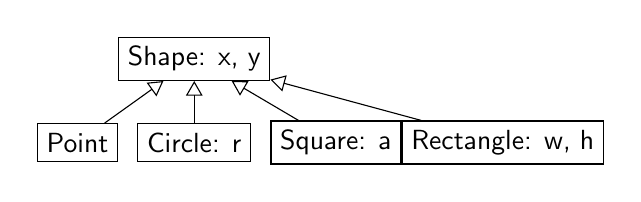
\begin{tikzpicture}
\matrix [ampersand replacement=\&,row sep=5mm] { 
	\&	\node [rectangle,draw] (shape) {\sf Shape: x, y} ; \\
\node [rectangle,draw] (point) {\sf Point}; \&
\node [rectangle,draw] (circle) {\sf Circle: r}; \&
\node [rectangle,draw] (square) {\sf Square: a} ;\&
\node [rectangle,draw] (rect) {\sf Rectangle: w, h};\\
};
\draw [open triangle 60-] (shape) -- (point);
\draw [open triangle 60-] (shape) -- (circle);
\draw [open triangle 60-] (shape) -- (square);
\draw [open triangle 60-] (shape) -- (rect);
\end{tikzpicture}
}
%\begin{tabular}{llll}
%& \rnode{shape}{\psframebox{Shape: x, y}} \\[2em]
%\rnode{point}{\psframebox{Point: }} &
%\rnode{circle}{\psframebox{Circle: r}} &
%\rnode{square}{\psframebox{Square: a}} &
%\rnode{rectangle}{\psframebox{Rectangle: w, h}} \\
%\end{tabular}
%\ncline{-}{shape}{point}
%\ncputicon[xunit=0.5,yunit=0.5]{umlHerit}
%\ncline{-}{shape}{circle}
%\ncputicon[xunit=0.5,yunit=0.5]{umlHerit}
%\ncline{-}{shape}{square}
%\ncputicon[xunit=0.5,yunit=0.5]{umlHerit}
%\ncline{-}{shape}{rectangle}
%\ncputicon[xunit=0.5,yunit=0.5]{umlHerit}
%}
\end{itemize}
\end{frame}


\defverbatim[colored]\codehaskinh{
\begin{lstlisting}[language={Haskell},escapechar=\#]
import Hugs.Trex; -- Only in -98 mode!!!

type Shape = Rec (x::Int, y::Int)
type Circle = Rec (x::Int, y::Int, r::Int)
type Square = Rec (x::Int, y::Int, w::Int)
type Rectangle = Rec (x::Int, y::Int, w::Int, h::Int)

move (x=_,y=_|rest) b c = (x=b,y=c|rest)

(a::Shape)=(x=12,y=24)
(b::Circle)=(x=12,y=24,r=10)
(c::Square)=(x=12,y=24,w=4)
(d::Rectangle)=(x=12,y=24,w=10,h=5)

Main> move b 4 5
(r = 10, x = 4, y = 5)
Main> move c 4 5
(w = 4, x = 4, y = 5)
Main> move d 4 5
(h = 5, w = 10, x = 4, y = 5)
\end{lstlisting}}
\begin{frame}
Haskell extensible records (only works for Hugs and in 98 mode!!):
\begin{beamercolorbox}{hexample}
\codehaskinh
\end{beamercolorbox}
\end{frame}

\begin{frame}
\frametitle{Haskell Classes}
\begin{itemize}
\item Subtyping hierarchy based on classes
\item An instance implements interface functions of the class
\item Functions operating on classes (using interface functions) can be
defined
\item \ \\
{\scriptsize
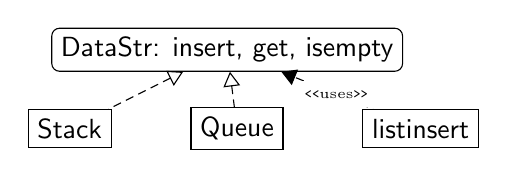
\begin{tikzpicture}
\node at (2,1) [rectangle,rounded corners=1mm,draw] (ds) {\sf DataStr: insert, get, isempty};
\node at (0,0) [rectangle,draw] (st) {\sf Stack} ; 
\node [rectangle,draw,right=of st] (qu) {\sf Queue} ; 
\node [rectangle,draw,right=of qu] (li) {\sf listinsert} ; 
\draw [open triangle 60-,densely dashed] (ds) -- (st);
\draw [open triangle 60-,densely dashed] (ds) -- (qu);
\draw [triangle 60-,densely dashed] (ds) -- node [fill=white,pos=0.6] {\tiny \texttt{<<}uses\texttt{>>}} (li);
\end{tikzpicture}
%\begin{tabular}{lll}
%\multicolumn{3}{c}{\rnode{datastr}{\psframebox[framearc=0.3]{DataStr: insert, get, isempty}}} \\[3em]
%\rnode{stack}{\psframebox{Stack}} &
%\rnode{queue}{\psframebox{Queue}} &
%\rnode{listinsert}{\psframebox{listinsert}} \\
%\end{tabular}\\[1em]
%\ncline[linestyle=dashed]{-}{datastr}{stack}
%\ncputicon[xunit=0.5,yunit=0.5]{umlHerit}
%\ncline[linestyle=dashed]{-}{datastr}{queue}
%\ncputicon[xunit=0.5,yunit=0.5]{umlHerit}
%\ncline[linestyle=dashed]{->}{listinsert}{datastr}
%\mput{\psframebox*{\tt <<uses>>}}
%
%\mbox{listinsert :: DataStr a $\Rightarrow$ (a v) $\rightarrow$ [v] $\rightarrow$ (a v)}
}\item Called \structure{interface} in OO programming

\end{itemize}
\end{frame}

\begin{frame}[fragile]
\frametitle{Haskell Default Class Hieararchy}
\scriptsize
\begin{columns}
\begin{column}{.56\textwidth}
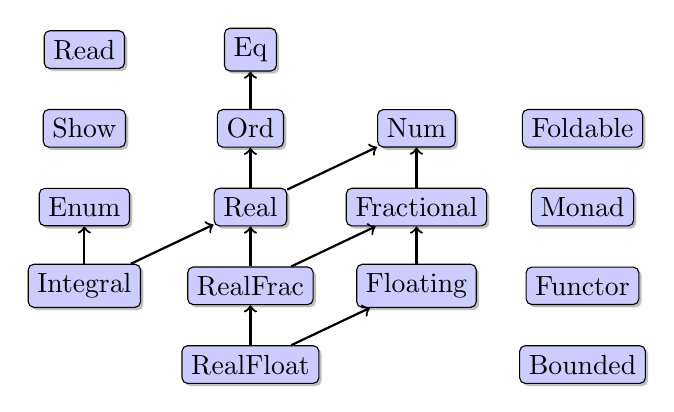
\begin{tikzpicture}
 \graph [grow up, branch right=6em, full/.style={rectangle,draw, fill=blue!20!white,
         rounded corners=2pt, drop shadow={shadow xshift=1pt, shadow yshift=-1pt}},
         edges={thick}]
        { dummy2 [as={}] -!- Integral [full] -> Enum  [full] -!- Show [full] -!- Read [full];
          RealFloat [full] -> RealFrac [full] -> Real [full] -> Ord [full] -> Eq [full];
          dummy [as={}] -!- Floating [full] -> Fractional [full]  -> Num [full];
          Bounded [full] -!- Functor [full] -!- Monad [full] -!- Foldable [full];
          Num <- Real;
          RealFrac -> Fractional;
          RealFloat -> Floating;
          Real <- Integral;
        };
\end{tikzpicture}
\end{column}
\begin{column}{.44\textwidth}
\begin{beamercolorbox}{hexample}
\begin{lstlisting}[language=Haskell,basicstyle=\tiny\tt]
Eq :  (==),(/=)

Ord: (<=), compare

Num: (+), (-), (*), negate, abs, 
     signum, fromInteger

Real: toRational

Fractional: (/), recip, fromRational

RealFrac: truncate, round, ceiling,..

Enum: succ, pred, toEnum fromEnum,...

Integral: quot, rem, div, mod,
   toInteger, divMod, quotRem

Floating: pi, exp, log, sin, (**),
          cos, asin, sinh, ...

RealFloat: floatRadix, exponent, 
  isNaN, isIEEE, decodeFloat,...

Show: show
\end{lstlisting}
\end{beamercolorbox}
\end{column}
\end{columns}
\end{frame}

\defverbatim[colored]\codehaskclass{
\begin{lstlisting}[language={Haskell},escapechar=\#]
class DataStr a where
    insert :: (a v) -> v -> (a v)
    get :: (a v)-> Maybe (v,(a v))
    isempty :: (a v) -> Bool

instance  DataStr Stack where
    insert x v = push v x
    get x = pop x
    isempty Empty = True
    isempty _ = False

instance DataStr Queue where
    insert x v = enqueue v x
    get x = dequeue x
    isempty EmptyQ = True
    isempty _ = False

insertlist :: DataStr a =>  (a v) -> [v] -> (a v)
insertlist x [] = x
insertlist x (el:rest) = insertlist  (insert x el) rest

data Stack a = Empty | St [a] deriving Show
data Queue a = EmptyQ | Qu [a] deriving Show
\end{lstlisting}}
\begin{frame}
\begin{beamercolorbox}{hexample}
\codehaskclass
\end{beamercolorbox}
\end{frame}



\subsection{Parametric Polymorphism}
\begin{frame}
\frametitle{Parametric Polymorphism}
 \begin{itemize}[<+->]
  \item \structure{Polymorphic} types: A value can have multiple types. Functions operate 
 on multiple types \structure{uniformly}
  \item \texttt{identity x = x}   function. type:	$\alpha \rightarrow \alpha$ \\
	\texttt{identity 4} : 4, \texttt{identity "ali"} : "ali" , \texttt{identity (5,"abc")} : (5,"abc") \\
	$int \rightarrow int$, $String \rightarrow String$, $int\times String \rightarrow int\times String$
 \item	\texttt{compose f g x = f (g x)} function\\
 type:  $(\beta \rightarrow \gamma) \rightarrow (\alpha \rightarrow \beta) \rightarrow \alpha \rightarrow \gamma$ \\
\texttt{compose square double 3} : 36,\\
$(int \rightarrow int) \rightarrow (int \rightarrow int) \rightarrow int \rightarrow int$.\\
\texttt{compose listsum reverse [1,2,3,4]} : 10 \\
$([int] \rightarrow int) \rightarrow ([int] \rightarrow [int]) \rightarrow [int] \rightarrow int$
 \end{itemize}
\end{frame}

\begin{frame}
 \begin{itemize}
  \item \texttt{\scriptsize filter f [] = []  \\
filter f (x:r) = if (f x) then x:(filter f r) else (filter r)}\\
 $(\alpha \rightarrow Bool) \rightarrow [\alpha] \rightarrow [\alpha]$\\
 \texttt{filter ((<) 3) [1,2,3,4,5,6]} : [4,5,6] \\
$(int \rightarrow Bool) \rightarrow [int] \rightarrow [int]$ \\
 \texttt{filter identity [True, False, True, False]} : [True,True] \\
 $(Bool \rightarrow Bool) \rightarrow [Bool] \rightarrow [Bool]$
\item Operations are same, types are different.
\item Types with type variables: \structure{polytypes}
\item Most functional languages are polymorphic
\item Object oriented languages provide polymorphism through inheritance
\end{itemize}
\end{frame}

\defverbatim[colored]\codeoverCpp{
\begin{lstlisting}[language={C++},escapechar=\#]
typedef struct Comp { double x, y; } Complex;
double #\color{orange}mult#(double a, double b) { return a*b; }
Complex #\color{green}mult#(Complex s, Complex u) {
    Complex t;
    t.x = s.x*u.x - s.y*u.y;
    t.y = s.x*u.y + s.y*u.x;
    return t;
}
Complex a,b; double x,y; ... ; a=#\color{green}mult#(a,b) ; x=#\color{orange}mult#(y,2.1);
\end{lstlisting}}
\section{Overloading}
\begin{frame}
\frametitle{Overloading}
\begin{itemize}
 \item \structure{Overloading}: Using same identifier for multiple places in same scope
 \item Example: Two different functions, two distinct types, same name.
 \item Polymorphic function: one function that can process multiple types.
 \item C++ allows overloading of functions and operators.
\begin{beamercolorbox}{cexample}
\codeoverCpp
\end{beamercolorbox}
\end{itemize}
\end{frame}

\begin{frame}
 \begin{itemize}
  \item Binding is more complicated. not only according to name but \alert{according to name
  and type}
  \item Function type:\\[.7em]
	\texttt{\tikz [remember picture,overlay] \matrix [anchor=west,rounded corners=2mm,thick,rectangle,draw=green!50!black,ampersand replacement=\&] (condep) {
			\node [rectangle,draw=orange!80!black,thick] (conind) { name : {\em parameters\/}}; \&
				\node {$\rightarrow$ \em result\/};\\};}\\[1em]
%	\texttt{\rnode{condep}{\psframebox[linecolor=green!50!black,framearc=0.4]{
%\rnode{conindep}{\psframebox[linecolor=orange!80!black,framearc=0.4]{
%name : {\em parameters\/}}} $\rightarrow$ {\em result}}}}
  \item \structure{Context dependent overloading}:
\begin{tikzpicture} [overlay,remember picture] 
\node (here) {}; \draw [<-,thick,black,green!50!black] (condep.south east) |- (here) ;
\end{tikzpicture}\\
 Overloading based on function
  name, parameter type and return type.
  \item \structure{Context independent overloading} : 
\begin{tikzpicture} [overlay,remember picture] 
\node (here) {}; \draw [->,thick,black,orange!80!black] (here) -| +(4,3) -| (conind) ;
\end{tikzpicture}\\
 Overloading based on
  function name and parameter type. No return type!
%  \ncbar[linecolor=orange!80!black,angleA=180]{->}{conindepp}{conindep}
%  \ncbar[linecolor=green!50!black]{->}{condepp}{condep}
 \end{itemize}
\end{frame}

\defverbatim[colored]\codecontdepCpp{
\begin{lstlisting}[language={C++},escapechar=\#]
int f(double a) { ....#\color{orange}\circtxt{1}# }
int f(int a) { ....#\color{green!50!black}\circtxt{2}# } 
double f(int a) { ....#\color{violet}\circtxt{3}# }  
double x,y; 
int a,b;
\end{lstlisting}}
\begin{frame}
 \frametitle{Context dependent overloading}
\begin{itemize}
 \item Which type does the expression calling the function expects (context) ?
\begin{beamercolorbox}{cexample}
 \codecontdepCpp
\end{beamercolorbox}
 \item {\small
	\texttt{a=f(x)}; \only<2->{{\color{orange}\circtxt{1}} (x double)} \\
	\texttt{a=f(a)}; \only<3->{{\color{green!50!black}\circtxt{2}} (a int, assign int)} \\
	\texttt{x=f(a)}; \only<4->{{\color{violet}\circtxt{3}} 
				(a int, assign double)} \\
	\texttt{x=2.4+f(a)}; \only<5->{{\color{violet}\circtxt{3}} 
				(a int, mult double)} \\
	\texttt{a=f(f(x))}; \only<6->{
{\color{green!50!black}\circtxt{2}}({\color{orange}\circtxt{1}}) ( x double, f(x):int, assign int)}  \\
	\texttt{a=f(f(a))}; \only<7->{
{\color{green!50!black}\circtxt{2}}({\color{green!50!black}\circtxt{2}}) or
{\color{orange}\circtxt{1}}({\color{violet}\circtxt{3}}) ???
}  
}
\item Problem gets more complicated. (even forget about coercion)
\end{itemize}
\end{frame}

\begin{frame}
\frametitle{Context independent overloading}
 \begin{itemize}
  \item Context dependent overloading is more expensive. 
  \item Complex and confusing. Useful as much?
  \item Most overloading languages are context independent.
  \item Context independent overloading forbids {\color{green!50!black}\circtxt{2}} and
  {\color{violet}\circtxt{3}} functions defined together.
  \item ``\texttt{name: parameters}'' part should be unique in 
  ``\texttt{\small name: parameters $\rightarrow$ result}'', in the same scope
\item Overloading is not much useful. So languages avoid it.
\begin{alertblock}{Use carefully:}
Overloading is useful only for functions doing same operations. Two functions with different
purposes should not be given same names. Confuses programmer and causes errors
\end{alertblock}
\item Is variable overloading possible? What about same name for two types?
\end{itemize}
\end{frame}

\defverbatim[colored]\codecoerC{
\begin{lstlisting}[language={C++},escapechar=\#]
double x;     int k;
x = k+4.2;     /* x = (double) k + 4.2 */
k = x+3.45;    /* k=(int) (x+3.45); */
k = x+2;       /* k=x+(double)2; */
k = x+k-2;     /* k=(int)(x+ (double)k - (double)2) ; */
\end{lstlisting}}
\section{Coercion}
\begin{frame}
\frametitle{Coercion}
 \begin{itemize}
  \item Making implicit type conversion for ease of programming.
\begin{beamercolorbox}{cexample}
\codecoerC
\end{beamercolorbox}
 \item C makes $int \leftrightarrow double$ coercions and pointer coercions (with warning)
 \item Are other type of coercions are possible? (like  A * $\rightarrow$ A, A $\rightarrow$ A *
 ). Useful?
 \item May cause programming errors: \texttt{x=k=3.25} : \texttt{x} becomes 3.0 
 \item Coercion + Overloading: too complex.
 \item Most newer languages quit coercion completely (\structure{Strict type checking})
 \end{itemize}
\end{frame}
\section{Type Inference}
\begin{frame}
\frametitle{Type Inference}
\begin{itemize}
\item Type system may force user to declare all types (C and most compiled imperative
languages), or
\item Language processor infers types. How?
\item Each expression position provide information (put a constraint)
on type inference:
\begin{itemize}
\item Equality $e=x, x::\alpha, y::\beta \;\Rightarrow\; \alpha\equiv\beta$
\item Expressions $e=a+f\;x \;,
+::Num \rightarrow Num \rightarrow Num 
\;\Rightarrow\;$ \\
$a::Num, 
f::\alpha \rightarrow Num,
e::Num$
\item Function application $e=f\;x \;\Rightarrow \; e::\beta, x::\alpha,
f::(\alpha \rightarrow \beta)$ 
\item Type constructors $f\;(x:r) = t \;\Rightarrow \; x::\alpha, t::\beta,
f::([\alpha] \rightarrow \beta)$
\end{itemize}
\item Inference of all values start from the most general type (i.e: any type
$\alpha$)
\item Type inference finds the \structure{most general type} satisfying the
constraints.
\end{itemize}
\end{frame}

\begin{frame}[fragile]
\frametitle{Inferring Type from Initializers}
\begin{itemize}
\item C++11 \lstinline{auto} type specifier gets type from initializer or return expression.
\item C++11 \lstinline{decltype(varexp)} gets type same as the variables declared type\\[.5em]
\begin{beamercolorbox}{cexample}
\begin{lstlisting}[language=C++]
auto f(int a) {  
   return a/3.0;  // double, function becomes double
}  
struct P { double x, y;} *pptr;

decltype(pptr->x) xval; // double since pptr->x is double

auto v = (P)({ 2.0, 4.0}); // initializer is P typed
auto t = f(3);    // f(3) returns double so t is double
\end{lstlisting}
\end{beamercolorbox}
\item GCC has \lstinline!typeof(expr)!, some other dialects have \lstinline!__typeof__(expr)! macro having a similar mechanism in C.
\end{itemize}
\end{frame}

\begin{frame}
\frametitle{Summary}
\begin{itemize}
\item Monomorphic vs Polymorphic types
\item Subtyping
\item Inheritence
\item Overloading
\item Parametric polymorphism
\item Coercion
\item Type Inference
\end{itemize}
\end{frame}
\end{document}
